\section{Low T PL}

\subsection{Introduction}

As the temperature of the semiconductor goes down the number of charge carriers decreases. Because of this in $WS_2$ the number of electrons is expected to be lower at low temperatures. Additionally as the temperature drops the peak broadening due to temperature effects i.e. Gaussian broadening decreases. At room temperature the thermal energy is equal to about 25 meV which limits the smallest possible width of the peak and therefore the resolution. Both of those effects should result in the peak at low temperatures to be overall weaker and more narrow than that at the room temperature. Additionally the lower electron density should result in lower population of trions. Due to lower temperature the electron and hole mobility should also decrease and cause the excitons to be more often trapped at defects sites also known as bound excitons.

\subsection{Experimental}



\subsection{Results}

The PL measurements were taken from the $WS_2$ monolayer on $Si/SiO_2$ sample at different conditions. As seen in Figure \ref{fig:LowTPLComparison} the PL from has been measured in the same spot at lower pressure ($2 \times 10^{-2}$) and different temperatures, room temperature and liquid nitrogen ($LN_2$) temperature ($-196 \degree C$). The PL from that spot at room temperature is centred at 1.957 eV and has FWHM of 44.3 meV. After lowering the temperature to that of $LN_2$ i.e. $-196 \degree C$ the PL measurement was taken again and the intensity of the peak was found to be about 0.81 that of the RT. Additionally the position of the PL at lower temperature was found to be 1.969 eV and the FWHM was 37.9 eV.

\begin{figure}[!ht]
	\begin{center}
		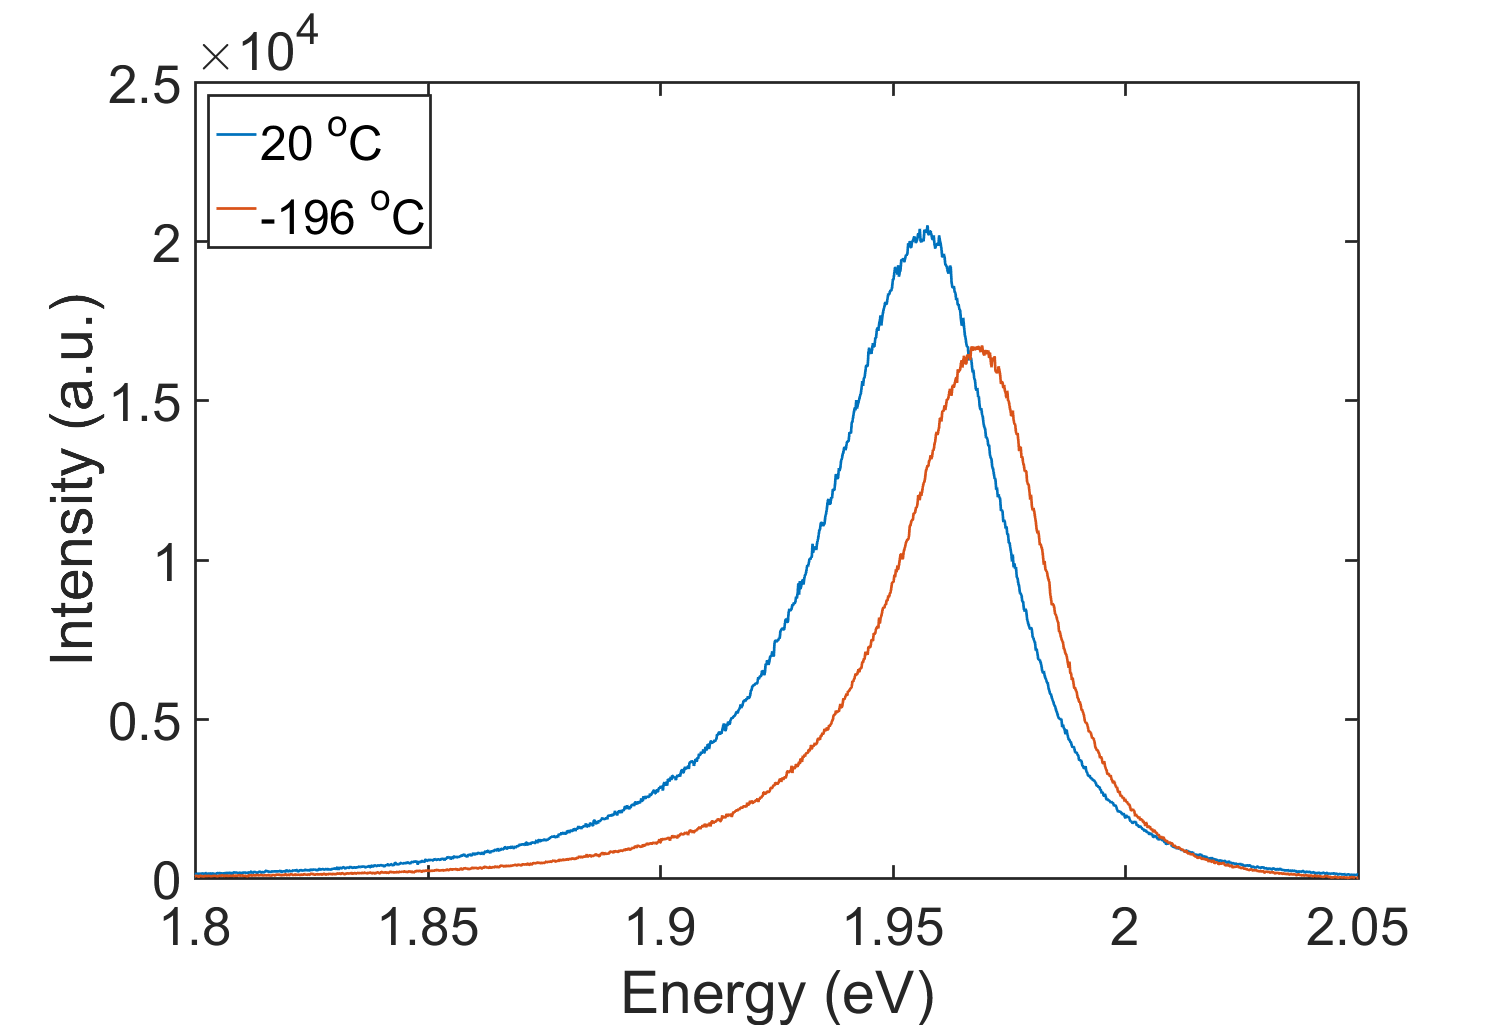
\includegraphics[scale=0.4]{LowT/LowTPLComparison.png}
		\caption{PL spectra of samples at room temperature and $LN_2$ temperature at $2 \times 10^{-2}$ mbar}
		\label{fig:LowTPLComparison}
	\end{center}
\end{figure}

The PL spectra were then fitted with 2 peaks to resolve the trions and excitons. The results can be seen in Figure \ref{fig:LowTPLDeconvolution}. Similarly the PL spectrum from room temperature has been fitted with two peaks. The intensity ratio between the exciton and trion in the low temperature sample is about 4, while at the room temperature it is 3. The FWHM of the exciton peak also lowers from 36 meV to about 32 meV.

This indicates that indeed as the temperature is lowered the FWHM of the PL peak and especially the exciton component also lowers. However the difference between the FWHM at room temperature and low temperature is not as big as expected if temperature was the main contributor to the peak broadening. For room temperature a thermal energy contribution should be about 25 meV while at $LN_2$ temperature (77 K) the contribution should be about 6 meV. 

\begin{figure}[!ht]
	\begin{center}
		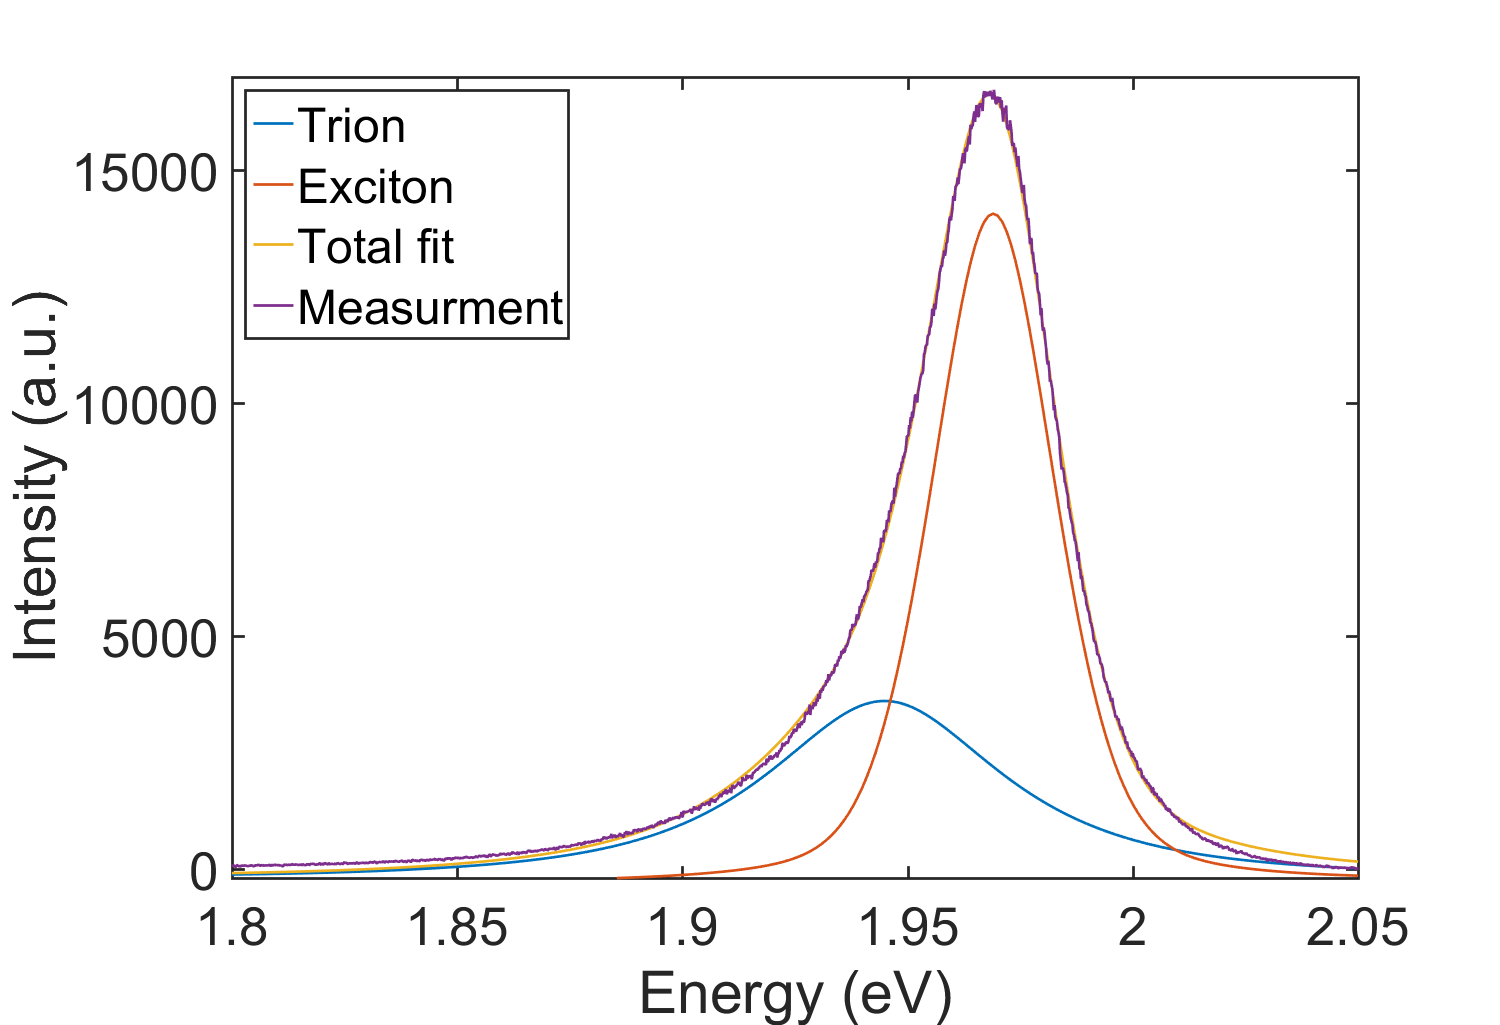
\includegraphics[scale=0.4]{LowT/LowTPLDeconvolution.png}
		\caption{PL spectra at low temperature with trions and excitons components resolved}
		\label{fig:LowTPLDeconvolution}
	\end{center}
\end{figure}